%% results.tex — Section 4: Measuring Learning Loss

\subsection{Descriptive Evidence}
\label{subsec:descriptive}

Table~\ref{tab:descriptive} reports mean test scores, participation rates, and
sample counts for the 2018 and 2021 monitoring waves. Scores are standardised
relative to the 2018 national distribution, so the 2018 mean is zero by
construction. Between waves, the mean mathematics score fell by 0.11~SD and
the mean reading score by 0.10~SD.

To convert these gaps to instructional time, I use the fourth-grade
learning-growth benchmarks from \citet{hill2008empirical}: 0.52~SD per school
year in mathematics and 0.36~SD per year in reading. The observed declines
correspond to roughly 0.21 school years lost in mathematics and 0.28 school
years lost in reading. These benchmarks are derived from US data and are not
calibrated to Ukraine's curriculum or student population; I treat the
school-year conversions as illustrative rather than precise.

Test participation declined between waves. The share of enrolled students who
sat the mathematics assessment fell from 90.8 to 85.8~percent, a drop of
five percentage points representing approximately 720 fewer tested pupils.
Reading participation followed a similar pattern. Because non-participation
is unlikely to be random, these figures motivate the attrition analysis in
Section~\ref{sec:robustness}.

\begin{table}[htbp]
\centering
\caption{Test scores and participation before and after school closures}
\label{tab:descriptive}
\begin{tabular}{lccc}
\toprule
 & \textbf{2018} & \textbf{2021} & \textbf{Difference} \\
\midrule
\multicolumn{4}{l}{\textit{Panel A: Mathematics}} \\
\quad Score (SD units)    & 0.00   & $-$0.11 & $-$0.11 \\
                          & (1.00) & (1.07)  & (0.07) \\
\quad Proportion tested   & 0.908  & 0.858   & $-$0.051 \\
\quad Tested              & 4,501  & 3,781   & $-$720 \\
\quad Enrolled            & 4,956  & 4,409   & $-$547 \\
\addlinespace
\multicolumn{4}{l}{\textit{Panel B: Reading}} \\
\quad Score (SD units)    & 0.00   & $-$0.10 & $-$0.10 \\
                          & (1.00) & (1.03)  & (0.06) \\
\quad Proportion tested   & 0.914  & 0.857   & $-$0.057 \\
\quad Tested              & 4,506  & 4,143   & $-$363 \\
\quad Enrolled            & 4,928  & 4,832   & $-$96 \\
\bottomrule
\end{tabular}
\begin{tablenotes}
\small
\item \textit{Notes}: Score rows report weighted means with weighted standard
deviations in parentheses. The Difference column reports 2021 minus 2018;
for test scores, the standard error of the difference (in parentheses) is
from a weighted regression with standard errors clustered at the school level.
Proportion tested equals tested divided by enrolled. Counts are unweighted.
\end{tablenotes}
\end{table}

Figure~\ref{fig:density} plots weighted kernel density estimates of standardised
scores in each wave. Both distributions shifted left between 2018 and 2021,
with the overall shape remaining stable---a pattern consistent with a broad
downward shift rather than losses concentrated at particular points of the
distribution.

\begin{figure}[htbp]
\centering
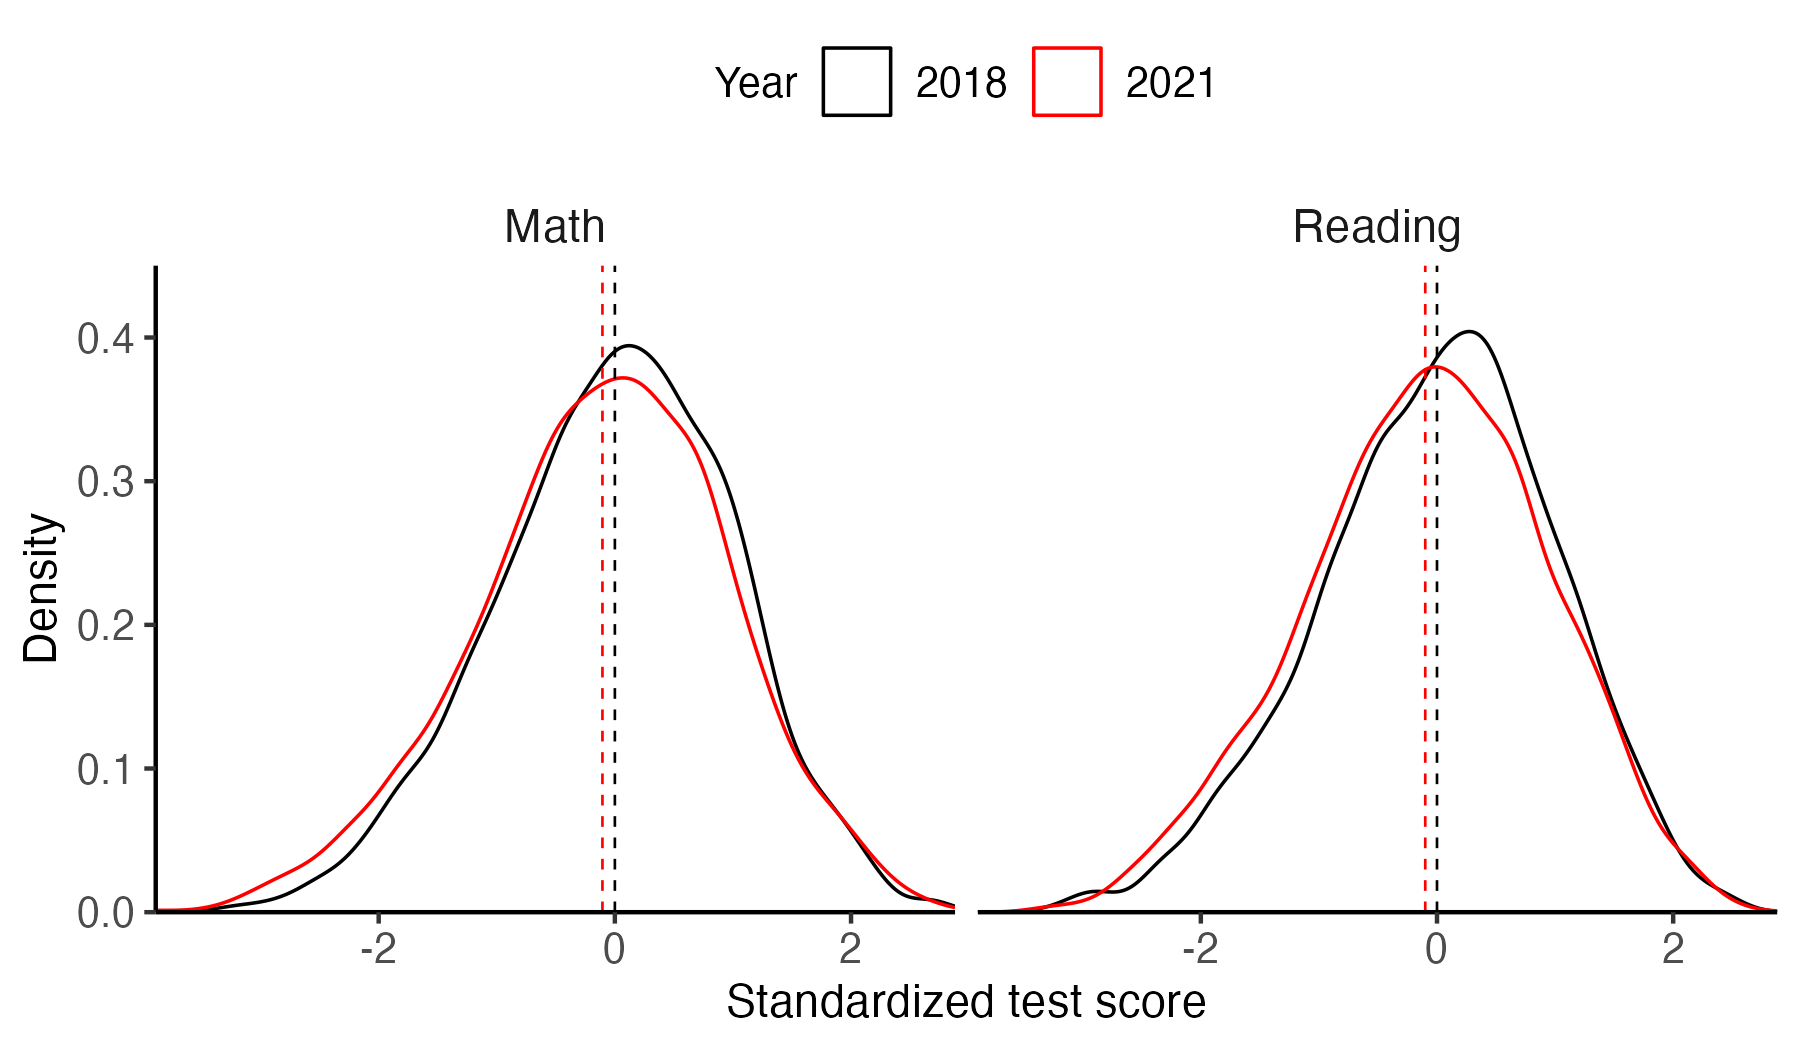
\includegraphics[width=\textwidth]{../Figures/score_distributions.png}
\caption{Distribution of standardised test scores in mathematics and reading,
2018 and 2021}
\label{fig:density}
\begin{tablenotes}
\small
\item \textit{Notes}: Weighted kernel density estimates. Scores are standardised
relative to the 2018 weighted mean and standard deviation. Dashed vertical lines
mark weighted means in each year.
\end{tablenotes}
\end{figure}

\subsection{Regression Specification}
\label{subsec:specification}

To estimate the cross-cohort change in achievement, I estimate:

\begin{equation}
Y_{irt} = \alpha_r + \beta_1 \cdot \mathit{May2021}_t
          + \mathbf{X}'_{irt} \boldsymbol{\beta}_2 + \varepsilon_{irt},
\label{eq:main}
\end{equation}

\noindent where $Y_{irt}$ is the standardised test score for student~$i$ in
region~$r$ and year~$t$; $\alpha_r$ are region fixed effects; $\mathit{May2021}_t$
is an indicator equal to one for the 2021 wave; and $\mathbf{X}_{irt}$ is a
vector of student and household characteristics. The preferred specification
includes the child's age in months, gender, an indicator for rural residence,
school-type dummies, books-at-home categories, and SES tertile dummies with a
separate indicator for missing SES information. All regressions use sampling
weights and cluster standard errors at the school level.

The coefficient $\beta_1$ identifies the cross-cohort difference in achievement
conditional on region fixed effects and observables. I interpret it as the
COVID-19-associated learning loss under the assumption that, absent the pandemic,
the 2021 cohort would have achieved at the same level as the 2018 cohort after
conditioning on region and observable characteristics. The central threat to this
interpretation is differential attrition across waves; I examine this in
Section~\ref{sec:robustness}.

\subsection{Results}
\label{subsec:main_results}

Table~\ref{tab:main} presents estimates of Equation~(\ref{eq:main}) across three
progressively richer specifications. Column~(1) includes only the wave indicator
and region fixed effects. Column~(2) adds student demographics and school type.
Column~(3) adds books at home and SES tertiles.

The estimated gap is stable across specifications. In column~(1), the 2021
mathematics cohort scores 0.105~SD below the 2018 cohort; in the preferred
column~(3), the estimate is $-$0.091~SD (SE~=~0.050). Reading estimates follow
the same pattern: $-$0.099~SD in column~(1) and $-$0.099~SD (SE~=~0.040) in
column~(3). Adding a rich set of demographic and household controls changes the
estimates by at most 0.01~SD, indicating that observable differences between
cohorts account for almost none of the raw gap.

The covariate estimates in column~(3) reflect familiar achievement gradients.
Rural students score 0.379~SD lower in mathematics and 0.290~SD lower in
reading than urban students---the largest single predictor in both subjects.
Home learning resources matter: relative to households with 0--10 books, those
with 26--100 books score 0.234~SD higher in mathematics and 0.403~SD higher
in reading. SES is positively correlated with achievement in both subjects; in
reading the high-vs-low tertile gap reaches 0.124~SD. Gender differences
diverge sharply by subject: girls score 0.288~SD higher in reading but show no
significant difference in mathematics ($-$0.012~SD).

\begin{table}[htbp]
\centering
\caption{Cross-cohort achievement differences: Mathematics and Reading (2018 vs.\ 2021)}
\label{tab:main}
\resizebox{\textwidth}{!}{%
\begin{tabular}{lcccccc}
\toprule
 & \multicolumn{3}{c}{\textbf{Mathematics}} & \multicolumn{3}{c}{\textbf{Reading}} \\
\cmidrule(lr){2-4} \cmidrule(lr){5-7}
 & (1) & (2) & (3) & (1) & (2) & (3) \\
\midrule
2021 cohort indicator
  & $-$0.105  & $-$0.101$^{*}$  & $-$0.091$^{*}$
  & $-$0.099$^{*}$ & $-$0.089$^{*}$ & $-$0.099$^{**}$ \\
  & (0.067) & (0.056) & (0.050)
  & (0.059) & (0.046) & (0.040) \\
\addlinespace
School type: Gymnasium/Lyceum
  & & $0.233^{*}$  & $0.215^{**}$
  & & $0.328^{**}$ & $0.253^{*}$ \\
  & & (0.126) & (0.106) & & (0.148) & (0.142) \\
School type: Specialised
  & & 0.050   & $-$0.024
  & & 0.096   & 0.088 \\
  & & (0.100) & (0.092) & & (0.085) & (0.074) \\
Rural
  & & $-$0.447$^{***}$ & $-$0.379$^{***}$
  & & $-$0.363$^{***}$ & $-$0.290$^{***}$ \\
  & & (0.091) & (0.082) & & (0.089) & (0.077) \\
Age (months)
  & & 0.003 & 0.004 & & 0.000 & 0.002 \\
  & & (0.004) & (0.004) & & (0.004) & (0.004) \\
Female
  & & 0.017   & $-$0.012
  & & $0.318^{***}$ & $0.288^{***}$ \\
  & & (0.038) & (0.037) & & (0.043) & (0.040) \\
\addlinespace
Books 11--25
  & & & $0.142^{**}$ & & & $0.233^{***}$ \\
  & & & (0.065)     & & & (0.066) \\
Books 26--100
  & & & $0.234^{***}$ & & & $0.403^{***}$ \\
  & & & (0.056)      & & & (0.064) \\
Books 101--200
  & & & $0.271^{***}$ & & & $0.382^{***}$ \\
  & & & (0.078)      & & & (0.073) \\
Books $>$200
  & & & $0.221^{**}$ & & & $0.298^{***}$ \\
  & & & (0.090)     & & & (0.082) \\
Books missing
  & & & $-$0.603$^{***}$ & & & $-$0.403$^{***}$ \\
  & & & (0.140)         & & & (0.152) \\
\addlinespace
SES: Middle tertile
  & & & $0.091^{**}$ & & & 0.013 \\
  & & & (0.045)     & & & (0.046) \\
SES: High tertile
  & & & 0.067        & & & $0.124^{**}$ \\
  & & & (0.053)      & & & (0.050) \\
SES: Missing
  & & & $-$0.609$^{***}$ & & & $-$0.578$^{***}$ \\
  & & & (0.076)         & & & (0.055) \\
\addlinespace
Region fixed effects & No & Yes & Yes & No & Yes & Yes \\
Controls             & No & Yes & Yes & No & Yes & Yes \\
\midrule
Observations & 8,282 & 8,128 & 8,128 & 8,649 & 8,578 & 8,578 \\
$R^2$        & 0.000 & 0.137 & 0.217 & 0.000 & 0.130 & 0.203 \\
\bottomrule
\end{tabular}}% end resizebox
\begin{tablenotes}
\small
\item \textit{Notes}: Survey-weighted OLS regressions. The dependent variable is
standardised using the 2018 weighted mean and standard deviation (separately by
subject). Standard errors are design-based, accounting for survey stratification
and clustering at the school (PSU) level. Region fixed effects are included in
columns~(2)--(3). Column~(3) additionally includes books-at-home categories and
SES tertiles with a missing-category indicator. Reference categories: regular
school, 0--10 books at home, low SES tertile.
$^{*}p<0.10$, $^{**}p<0.05$, $^{***}p<0.01$.
\end{tablenotes}
\end{table}

Because the design compares repeated cross-sections, the estimates identify
population-level cohort differences rather than within-school changes. Under
the maintained assumption that the 2021 cohort would have performed similarly
to the 2018 cohort absent the pandemic, conditional on region and observables,
the 0.09--0.10~SD gap represents the COVID-19-associated learning shortfall.
Section~\ref{sec:robustness} tests the robustness of this interpretation
against differential attrition and compositional change.
